\documentclass[a4paper,12pt]{article}
\usepackage[english]{babel}
\usepackage[utf8]{inputenc}
\usepackage{amsmath, amsthm, amssymb, tikz}
\usetikzlibrary{decorations.pathreplacing}
\usepackage[a4paper,includeheadfoot,margin=2.54cm]{geometry}
\title{Experimentell Metodik}
%
\author{Zacharias Brohn\thanks{email: \texttt{zacbro-8@student.ltu.se}}\\  
        Elis Bergdahl\thanks{email: \texttt{elieba-4@student.ltu.sel}} \\
        Mikael Baer\thanks{email: \texttt{DinMejl}} \\
        ~ \\
        Luleå tekniska universitet \\ 
        971 87 Luleå, Sverige}
%
\date{\today}
%
\begin{document}
%
\maketitle
%
\begin{abstract}
\end{abstract}
%
\section{Inledning}
    Detta projekt har som syfte att undersöka volymflödet av materia genom smala, horisontella rör. I dessa undersökningar används endast vatten $(H_2O)$ men de matematiska beräkningar och metoder som har använts ska i teorin även vara korrekta för annan materia.
%
\section{Teori}
%
\subsection{Dimensionsanalys}
    En dimensionsanalys är en metod som tillämpas för att kontrollera att framtagna formler inte innehåller felaktiga variabler. Genomförande av metoden innebär att studera variablernas dimensioner på de ingående kvantiteter i formeln.
%
\subsection{Linjäresering}
    För en potensfunktion:
        \begin{align}
            Y = C \cdot x^a
        \end{align}
    Kan exponenten $a$ bestämmas med hjälp av logaritmering i höger- respektive vänsterled,
        \begin{align}
            ln Y = ln C + a \cdot ln x \implies Y = m + k \cdot X
        \end{align}
    Där:
        \begin{align}
            Y = ln y, k = a, X = ln x \text{ och } m = ln C
        \end{align}
    $Y$ plottas mot $X$, lutningen av grafen ges av exponenten $k$ och $m$ är linjens skärningspunkt i $Y$-axeln
%
\section{Metod}
%
\subsection{Genomförande}
    Vid genomförandet nyttjades en anordning av slangar, en vattenbehållare, ett glasrör och en vattenkran som vattenkälla enligt figur 1. Anordningen var monterad på en passande ställning. Totalt var fyra slangar dragna från vattenbehållaren som fungerade som huvudobjektet i anordningen. En slang fästes som en direktkoppling mellan vattenkranen och vattenbehållaren, en annan användes som överflödesskydd kopplad direkt till vasken, en som var kopplad till glasröret och den sista som med hjälp av en gänga i ena änden fungerade som fäste för teströren. På glasröret var en linjal monterad, en mätningsanordning som användes för att bestämma och kontrollera vattentrycket. Mest väsentligt var teströren, som var tio stycken. Rörens längd och diameter varierade och delades upp med hjälp av färger.

    
    \begin{figure}[h]
        \centering
        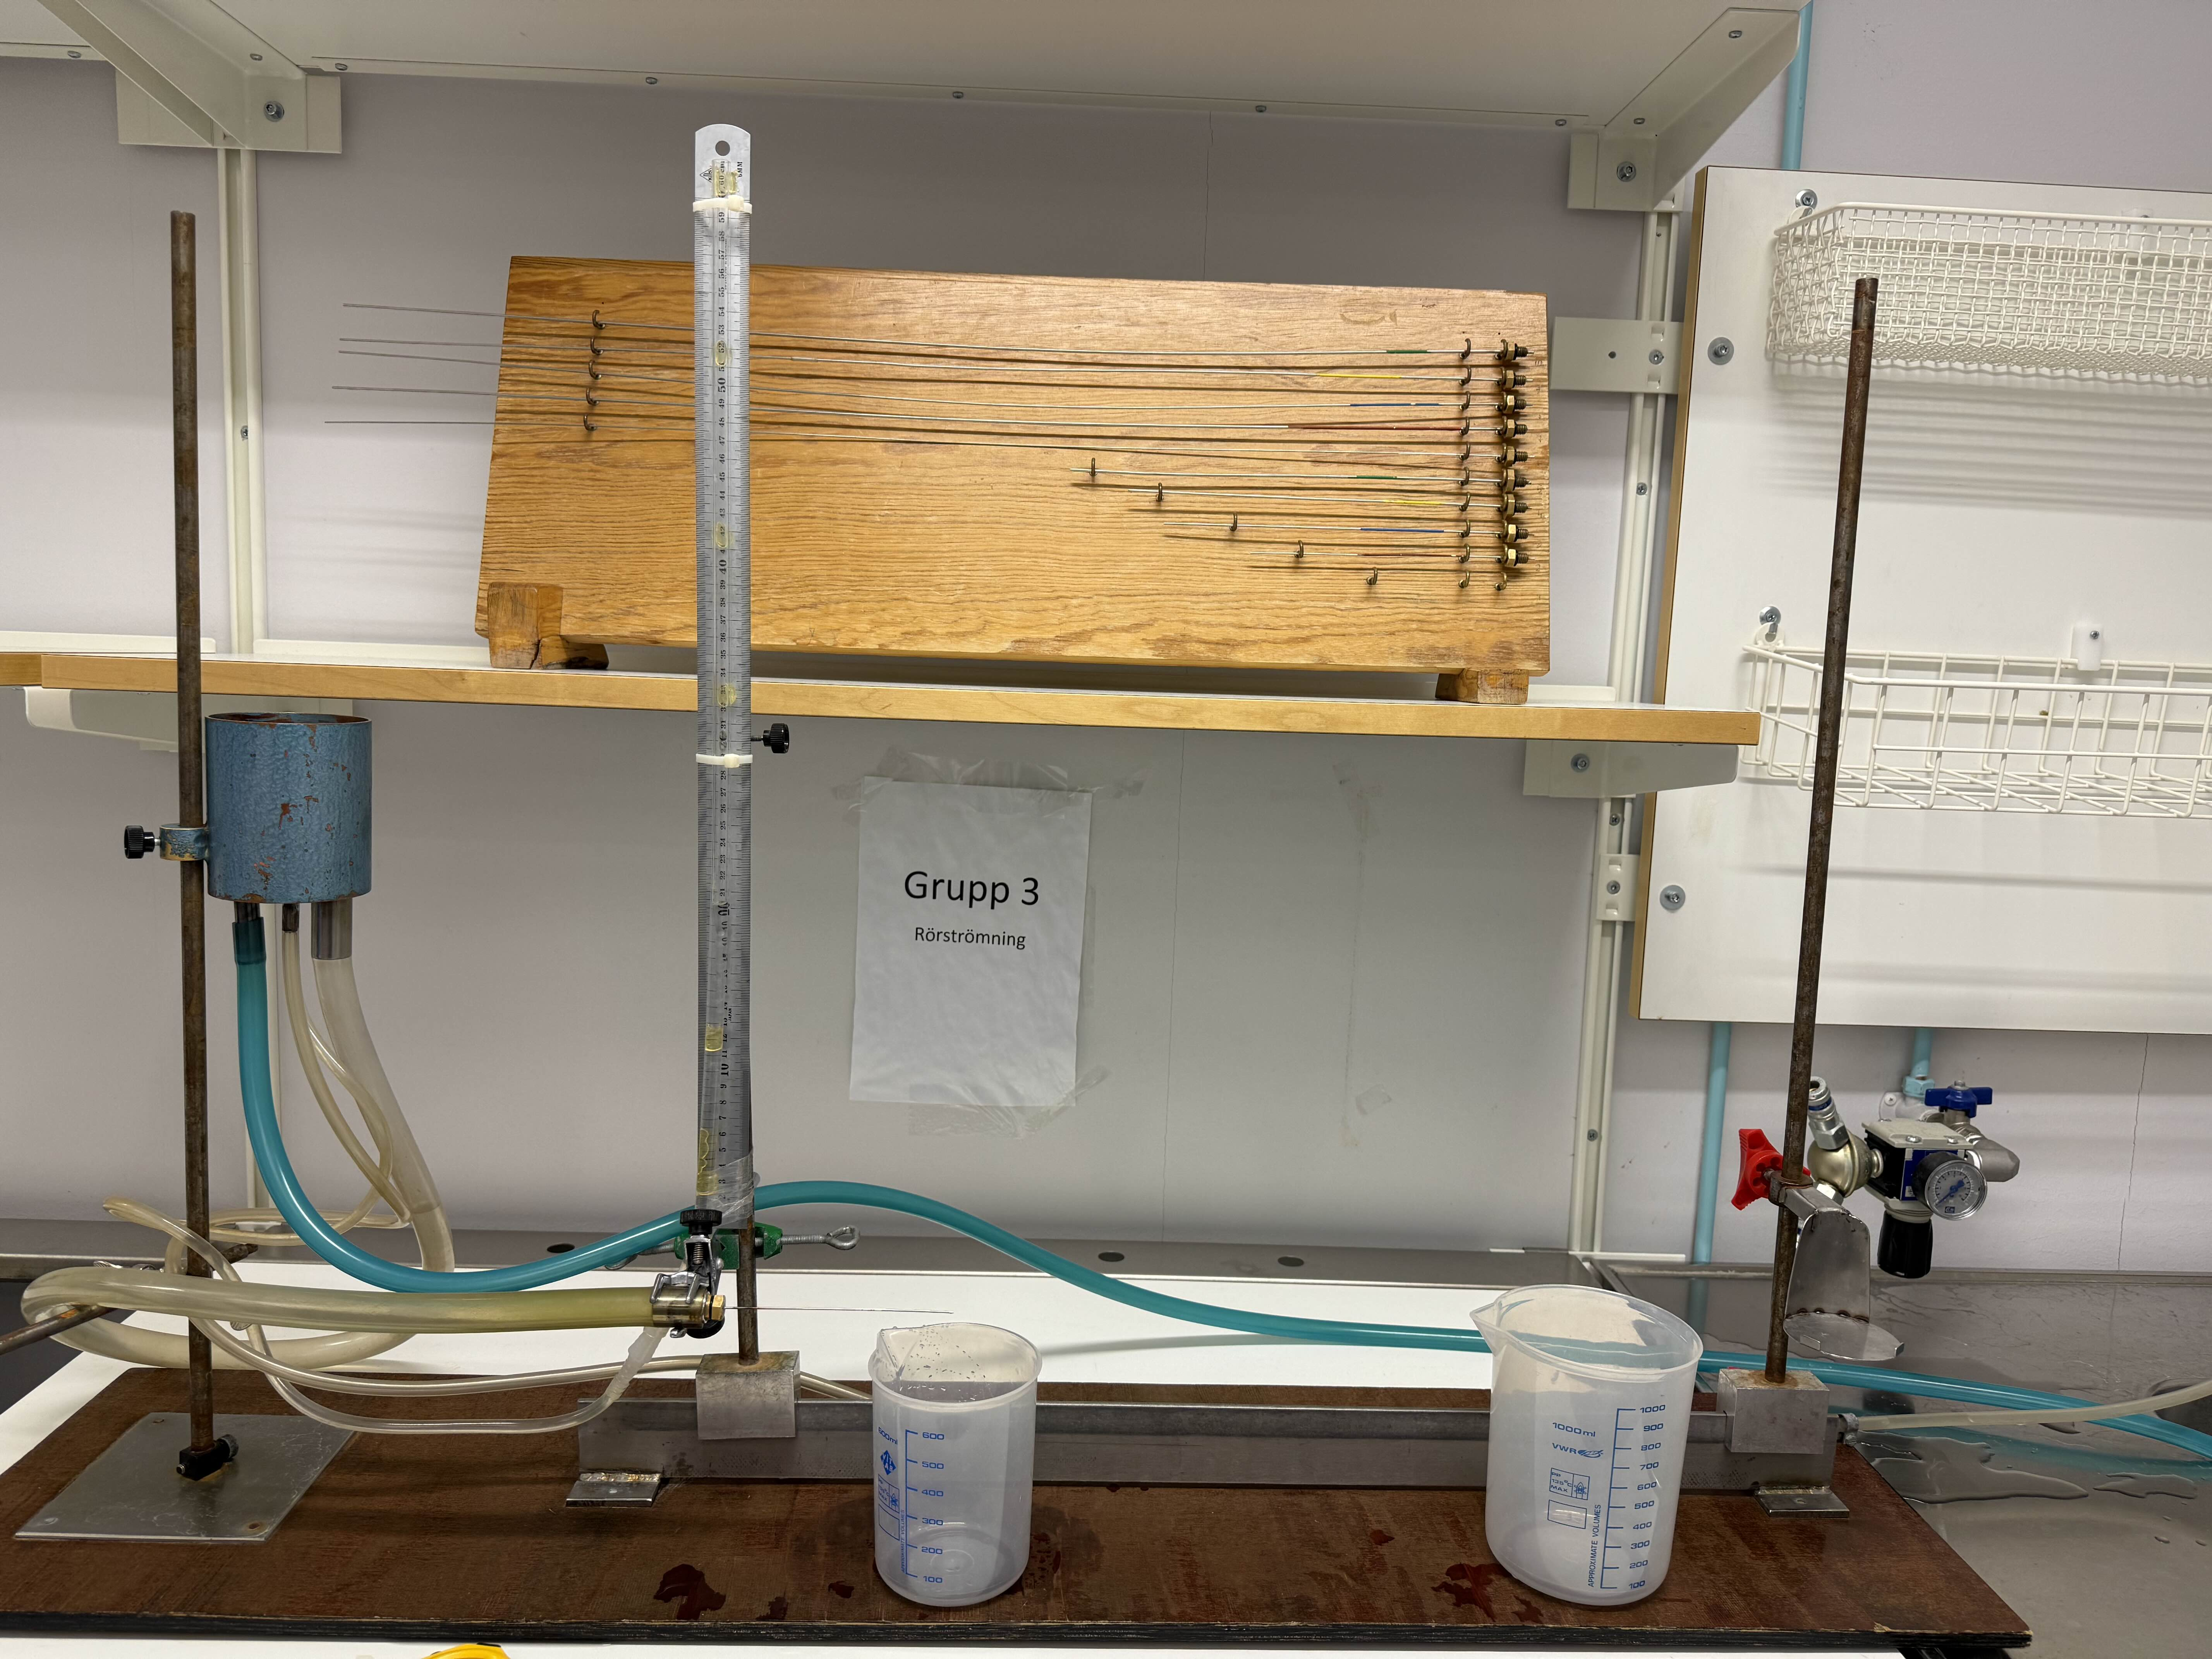
\includegraphics[width=0.5\textwidth]{Labb-yta.jpg}
        \caption{Laborationsanordningen.}
        \label{fig:experiment_setup}
    \end{figure}
    Med denna anordning kunde vi mäta vattenflödet genom att låta vattnet flöda genom röret en bestämd tid och sedan samla upp vattnet i en bägare som vägdes.
    Experimentet genomfördes genom att ett specifikt rör monterades beroende på vilken variabel som skulle mätas. Därefter vägdes bägaren, och kranen öppnades tills ett konstant vattenflöde uppnåddes. Vid behov kontrollerades vattentrycket genom att kolla på glasröret (förutom då trycket var den undersökta variabeln).
    När mätningen påbörjades placerades bägaren under utloppet, och tidtagningen startades samtidigt som vattenstrålen började rinna i bägaren. Alla mätvärden dokumenterades och samlades i ett Excel-ark för vidare analys. Totalt ändrades fyra variabler under mätningarna: rördiametern, rörlängden, vattentrycket och tiden då vattnet flödade.
\clearpage
\begin{table}[h!]
    \centering
    \begin{tabular}{|c|c|c|}
        \hline
            \textbf{Storhet} & \textbf{Betäckning} & \textbf{Dimension}\\ \hline
            Volymflöde & $Q$ & $L^3T^-1$\\ \hline
            Rörlängd & $l$ & $L$\\ \hline
            Rördiameter & $d$ & $L$\\ \hline
            Tid & $t$ & $T$\\ \hline
            Volym & $V$ & $L^3$\\ \hline
            Densitet* & $\rho$ & $ML^-3$\\ \hline
            Tyngdacceleration* & $g$ & $LT^-2$\\ \hline
            Viskositet* & $\mu$ & $ML^-1T^-1$\\ \hline
            Höjd i glasrör (vattentryck) & $h$ & $L$\\ \hline
    \end{tabular}
    \caption{Lista över variabler som användes i experimentet med storhet, betäckning och dimension. Variabler med * har varit oförandrade genom hela experimentet.}
    \label{tab:Variabellista}
\end{table}
\subsection{Material och noggranhet}
    Två bägare användes för att undvika onödigt spill av vatten, båda gjorda av plast Slangarna var gjorda av mjukt gummi och plast och var flexibela men inte så att de hindrade vattenflödet i något läge. Noggranheten för vattenmängden var 1 mm.
\end{document}
